\documentclass[11pt,a4paper]{article}
\usepackage[margin=25mm,headheight=15pt]{geometry}
\usepackage{fontspec}
\setmainfont{Latin Modern Roman}
\setsansfont{Latin Modern Sans}
\setmonofont[Scale=0.86]{Latin Modern Mono}
\usepackage{amsmath,amsthm}
\usepackage{unicode-math}
\setmathfont{Latin Modern Math}
\usepackage[expansion=false]{microtype}
\usepackage{graphicx,booktabs,longtable,array,enumitem,xcolor}
\usepackage{fancyhdr,lastpage,needspace}
\usepackage[unicode,colorlinks=true,linkcolor=teal,citecolor=teal,urlcolor=teal]{hyperref}
\definecolor{teal}{HTML}{176B73}
\definecolor{navy}{HTML}{17324D}
\definecolor{muted}{HTML}{56616A}
\hypersetup{pdftitle={Exact marginal crossover for a quartic Bose gas},
 pdfauthor={Research draft developed with ChatGPT},
 pdfsubject={Convergent Mellin expansion, rigorous summation, critical-temperature inversion, and uniform lattice corrections}}
\numberwithin{equation}{section}
\newtheorem{theorem}{Theorem}[section]
\newtheorem{proposition}[theorem]{Proposition}
\newtheorem{lemma}[theorem]{Lemma}
\newtheorem{corollary}[theorem]{Corollary}
\theoremstyle{definition}
\newtheorem{definition}[theorem]{Definition}
\newtheorem{remark}[theorem]{Remark}
\newcommand{\R}{\mathbb R}
\newcommand{\N}{\mathbb N}
\newcommand{\C}{\mathbb C}
\newcommand{\dd}{\,\mathrm d}
\newcommand{\Li}{\operatorname{Li}}
\newcommand{\con}{\mathrm{con}}
\newcommand{\latt}{\mathrm{lat}}
\newcommand{\e}{\mathrm e}
\newcommand{\Aconst}{\mathcal A}
\newcommand{\Bconst}{\mathcal B}
\newcommand{\Dconst}{\mathcal D}
\newcommand{\rad}{\mathcal R}
\newcommand{\gfour}{\Gamma(\tfrac14)}
\newcommand{\gthree}{\Gamma(\tfrac34)}
\setlength{\parindent}{1.1em}
\setlength{\parskip}{3pt}
\setlength{\emergencystretch}{2em}
\setlist{topsep=5pt,itemsep=3pt,parsep=0pt}
\pagestyle{fancy}
\fancyhf{}
\fancyhead[L]{\small\sffamily\color{muted}Exact marginal Bose crossover}
\fancyhead[R]{\small\sffamily\color{muted}Research draft}
\fancyfoot[L]{\footnotesize\color{muted}8 October 2026}
\fancyfoot[R]{\footnotesize\thepage\ /\ \pageref*{LastPage}}
\renewcommand{\headrulewidth}{0.3pt}
\raggedbottom
\allowdisplaybreaks[2]

\begin{document}
\hypersetup{pageanchor=false}
\begin{titlepage}
\thispagestyle{empty}
\vspace*{2mm}
{\sffamily\small\color{teal}ASYMPTOTIC ANALYSIS \quad / \quad MATHEMATICAL PHYSICS\par}
\vspace{6mm}
{\fontsize{29}{34}\selectfont\bfseries\color{navy}Exact marginal crossover\\[3mm]for a quartic Bose gas\par}
\vspace{7mm}
{\Large A convergent expansion, rigorous computation,\\[1mm]
and uniform lattice corrections\par}
\vspace{6mm}
{\large Research article and computational supplement\par}
\vspace{2mm}
{\color{muted}Developed and independently checked with ChatGPT\par}
{\color{muted}8 October 2026\quad\textbullet\quad Version 1.0\par}
\vspace{6mm}
\hrule
\vspace{6mm}
\noindent\small\textbf{Abstract.}
We sharpen the marginal logarithmic crossover formula of Łebek and
Jakubczyk, \emph{Physical Review A} \textbf{102} (2020), 013324,
by evaluating its previously unspecified next constant and proving a
convergent expansion with a sharp radius and an explicit remainder.
For
\[
 \Psi(u)=\int_{\R}\e^{-x^4-u x^2}\dd x,
 \qquad G(s)=\sum_{n\ge1}\frac{\Psi(s\sqrt n)}n,
\]
we establish
\[
 G(s)=\gfour\left(\log\frac1s+\frac\pi4+\frac32\log2\right)
 +\frac12\sum_{k\ge1}\frac{(-1)^k\Gamma(\frac14+\frac k2)
 \zeta(1-\frac k2)}{k!}\,s^k.
\]
The correction series has radius exactly $\sqrt{8\pi}$ and converges
absolutely on its convergence circle. In the published variable
$\theta=s^2/8$, the constant next to $\log(1/\theta)$ is exactly
$\pi/2$. A Mellin-contour estimate proves equality, including the
absence of an unaccounted exponentially small term.

The expansion yields a summation algorithm requiring
$O(\log(1/\varepsilon))$ special-function evaluations for absolute
accuracy $\varepsilon$, uniformly over positive stiffness, when combined
with an explicitly bounded large-stiffness tail. We derive a convergent
Lambert-$W$ expansion for the inverse critical temperature. Finally,
for a specified finite-range lattice dispersion, we prove an all-orders
low-temperature expansion uniform as the stiffness vanishes. Its first
two lattice coefficients give corrections to the inverse critical line
that dominate the exponentially small continuum stiffness corrections.
The package includes arbitrary-precision reference code,
outward-rounded Arb enclosures, independent quadrature, tests, and data.

\vfill
\noindent\small\color{muted}
\textbf{Scope.} The results are analytical theorems about explicitly defined
Bose integrals and their lattice realization. The logarithmic crossover
and its physical setting are prior work. This report provides a precise
quantitative strengthening; it makes no claim to resolve a famous open
conjecture or to establish the interacting Heisenberg model results in the
inspirational repository. Publication priority beyond the sources reviewed
has not been established. The proofs are not machine formalized.
\end{titlepage}
\hypersetup{pageanchor=true}

\tableofcontents
\clearpage

\section{The research target and the precise advance}
\label{sec:target}

The starting inspiration was the heat-kernel approach to lattice
corrections in Family 271 of the \texttt{openai/math} collection
\cite{OAIcatalog,OAIbloch}. In its elementary ideal-gas calculation, a
uniform expansion of a lattice heat kernel is evaluated at integer
multiples of inverse temperature and summed over those integers.
We ask what remains true when the quadratic coefficient in a direction
vanishes, so that the limiting dispersion becomes quartic and the Bose
sum reaches its marginal integrability threshold.

This question leads to a concrete published target. Section IV.2 of
Łebek--Jakubczyk \cite{LJ2020}, especially their equation (25), obtains the
leading logarithmic critical line for one quadratic and two quartic
directions, with a small positive quadratic stiffness in one of the
quartic directions. Their cutoff argument leaves the next, nonlogarithmic
coefficient unspecified. We replace that cutoff argument with an exact
Mellin calculation and control the contour remainder.

The methods themselves are classical. Harmonic sums and their Mellin
transforms are treated systematically in \cite{FGD1995}; convergent
exponential--Bessel expansions appear in \cite{Paris2020}, and numerical
acceleration of related Schlömilch sums in \cite{LintonBarnett2004}.
Paris's stated exponential--$K$ family has positive exponential damping
and a linked power/order parameter. The present sum has an independent
$n^{-3/4}$ weight and the cancellation boundary
$\e^{n\theta}K_{1/4}(n\theta)$. We do not attribute novelty to the general
Mellin method. The concrete additions here are the evaluated marginal
constant, the complete specialized convergent expansion and its
remainder, the inverse formulas, and a uniform transfer to a specified
lattice model.

\begin{table}[ht]
\centering\small
\begin{tabular}{>{\raggedright\arraybackslash}p{.27\linewidth}
>{\raggedright\arraybackslash}p{.29\linewidth}
>{\raggedright\arraybackslash}p{.34\linewidth}}
\toprule
Question & Established starting point & Result proved here\\
\midrule
Marginal continuum crossover & Leading $T\log(1/\theta)$ law in
\cite{LJ2020} & Exact constant $\pi/2$ and every correction coefficient\\[2mm]
Nature of the expansion & Cutoff asymptotic estimate & Convergent
series; sharp radius; explicit contour remainder\\[2mm]
Numerical evaluation & A slowly convergent positive Bessel sum &
Uniform logarithmic term count with rigorous tail control\\[2mm]
Inverse critical line & Logarithmic suppression of temperature &
Lambert-$W$ approximation and convergent correction recursion\\[2mm]
Actual lattice & Continuum low-energy description & All-orders
asymptotic expansion uniform in the degenerating stiffness\\
\bottomrule
\end{tabular}
\caption{The scope of the strengthening. ``Uniform logarithmic term count''
counts special-function evaluations, not bit operations.}
\label{tab:scope}
\end{table}

All subsequent results are proved from the displayed integral definitions.
No unverified top-level assertion from \texttt{openai/math} is an input.
The repository is cited for the research direction and the heat-kernel
organization of the calculation.

\section{Definitions, normalization, and the marginal obstruction}
\label{sec:setup}

\subsection{The quartic heat kernel and its harmonic sum}

For $u\ge0$, define
\begin{equation}
 \Psi(u)=\int_{\R}\exp(-x^4-u x^2)\dd x,
 \qquad \Psi(0)=\frac12\gfour.
 \label{eq:psi}
\end{equation}
For $u>0$, dropping the quartic term gives
\begin{equation}
 0<\Psi(u)\le\sqrt\pi\,u^{-1/2}.
 \label{eq:psibound}
\end{equation}
Consequently
\begin{equation}
 G(s)=\sum_{n=1}^{\infty}n^{-1}\Psi(s\sqrt n),\qquad s>0,
 \label{eq:G}
\end{equation}
converges, since it is at most
$\sqrt\pi s^{-1/2}\zeta(5/4)$. It is strictly decreasing in $s$.
At $s=0$, each heat-kernel factor is constant, and the harmonic sum
diverges. The small positive stiffness therefore regulates a real
logarithmic singularity; it cannot be set to zero inside the original sum.

The standard quartic integral also gives
\begin{equation}
 \Psi(u)=\frac{\sqrt u}{2}\e^{u^2/8}K_{1/4}(u^2/8).
 \label{eq:bessel}
\end{equation}
One may establish this from the integral representation of $K$ by
substitution, or verify that both sides solve the same differential
equation in $u$ and have the Gaussian large-$u$ normalization.
The heat-integral definition remains primary throughout the proofs.

\subsection{An exact continuum density}

We work in units with the three positive leading energy coefficients and
Boltzmann's constant normalized to one. Define, for $T,\delta>0$,
\begin{equation}
 N_{\con}(T,\delta)=\frac1{(2\pi)^3}\int_{\R^3}
 \frac{\dd x\dd y\dd z}
 {\exp((x^2+y^4+z^4+\delta z^2)/T)-1}.
 \label{eq:Ncon}
\end{equation}
Expanding the Bose denominator into its positive exponential series and
using Tonelli's theorem gives
\begin{equation}
 N_{\con}(T,\delta)=C_* T\,G(s),\qquad
 C_*:=\frac{\gfour}{16\pi^{5/2}},\qquad s:=\frac\delta{\sqrt T}.
 \label{eq:normalization}
\end{equation}
Indeed the $x$ integral is $\sqrt\pi(T/n)^{1/2}$, the $y$ integral is
$\frac12\gfour(T/n)^{1/4}$, and the $z$ integral is
$(T/n)^{1/4}\Psi(s\sqrt n)$. This explicitly checks every factor of two
and $\pi$.

The weighted dimension at $\delta=0$ is
$\frac12+\frac14+\frac14=1$. The zero-gap Bose integral is then exactly
at its logarithmic integrability threshold. For $\delta>0$, the last
direction is quadratic at sufficiently low energy and the weighted
dimension increases to $5/4$, making \eqref{eq:Ncon} finite.

\subsection{Connection with the published scaling variable}

Set
\begin{equation}
 \theta=\frac{s^2}{8},\qquad
 S(\theta)=\sum_{n\ge1}n^{-5/4}
 \sqrt{n\theta}\,\e^{n\theta}K_{1/4}(n\theta).
 \label{eq:Stheta}
\end{equation}
The exact identity
\begin{equation}
 S(\theta)=2^{1/4}\theta^{1/4}G(\sqrt{8\theta})
 \label{eq:Smap}
\end{equation}
connects our normalization to that of \cite{LJ2020}. For the general
dispersion $t_0(k_1a_0)^2+t(k_2a_0)^4+\tau(k_3a_0)^2+
\tau'(k_3a_0)^4$, replace
\begin{equation}
 s=\frac\tau{\sqrt{\tau' k_BT}},\qquad
 \theta=\frac{\tau^2}{8\tau' k_BT},
 \label{eq:units}
\end{equation}
and multiply the normalized density by
$[a_0^3\sqrt{t_0}\,t^{1/4}(\tau')^{1/4}]^{-1}$, using $k_BT$ for $T$.
For the imperfect gas of \cite{LJ2020}, the critical chemical potential
equals this ideal critical density times the mean-field coupling.
These are changes of scale, not additional interaction theorems.

\section{The exact convergent expansion}
\label{sec:main}

Put
\begin{equation}
 R_*:=\sqrt{8\pi},\qquad
 c_k:=\frac{(-1)^k}{2k!}\Gamma\left(\frac14+\frac k2\right)
                  \zeta\left(1-\frac k2\right)\quad(k\ge1).
 \label{eq:coeffs}
\end{equation}

\begin{theorem}[Exact expansion and a quantitative remainder]
\label{thm:main}
For every real $0<s\le R_*$,
\begin{equation}
 G(s)=\gfour\left(\log\frac1s+\frac\pi4+\frac32\log2\right)
       +\sum_{k=1}^{\infty}c_k s^k.
 \label{eq:main}
\end{equation}
The correction series has radius exactly $R_*$ as a complex power
series and converges absolutely for every $|s|=R_*$. For $j\ge1$, its
partial sum through degree $4j+1$ satisfies
\begin{equation}
 \left|G(s)-\gfour\left(\log\frac1s+\frac\pi4+\frac32\log2\right)
              -\sum_{k=1}^{4j+1}c_k s^k\right|
 \le B_j\left(\frac{s}{R_*}\right)^{4j+2},
 \label{eq:blockbound}
\end{equation}
where
\begin{equation}
 B_j=\frac{\sqrt\pi\,\zeta(2j+1)}
 {(4j+2)(2j+\tfrac14)^{1/4}}.
 \label{eq:Bj}
\end{equation}
The same finite-contour inequality is valid for every $s>0$, although its
right side no longer tends to zero as $j\to\infty$ when $s>R_*$.
\end{theorem}

There is an exact zero pattern:
\begin{equation}
 c_6=c_{10}=c_{14}=\cdots=0.
 \label{eq:zeropattern}
\end{equation}
The coefficient $c_2$ is not zero, because $\zeta(0)=-1/2$ is not a
trivial zeta zero.

\begin{corollary}[The missing constant]
\label{cor:missingconstant}
With $\theta$ as in \eqref{eq:Stheta}, for $0<\theta\le\pi$,
\begin{equation}
 S(\theta)=\frac{\gfour}{2^{3/4}}\theta^{1/4}
 \left[\log\frac1\theta+\frac\pi2
       +\sum_{k\ge1}d_k\theta^{k/2}\right],
 \label{eq:published}
\end{equation}
where
\begin{equation}
 d_k=\frac{(-1)^k8^{k/2}\Gamma(\frac14+\frac k2)
                    \zeta(1-\frac k2)}{k!\gfour}.
 \label{eq:dk}
\end{equation}
Thus the unspecified constant alongside the logarithm in the published
marginal expression is exactly $\pi/2$.
\end{corollary}

For compact physical formulas, define
\begin{equation}
 \Aconst:=\frac{\gfour^2}{32\pi^{5/2}},\qquad
 b_k:=\frac{2c_k}{\gfour},\qquad
 B(s):=\sum_{k\ge1}b_k s^k,\qquad
 \kappa:=8\e^{\pi/2}.
 \label{eq:AB}
\end{equation}
Then
\begin{equation}
 \boxed{N_{\con}(T,\delta)=\Aconst T
 \left[\log\frac{8T}{\delta^2}+\frac\pi2
                       +B(\delta/\sqrt T)\right].}
 \label{eq:physicalmain}
\end{equation}
This identity applies when $0<\delta/\sqrt T\le R_*$.
The first terms are
\begin{align}
 b_1&=-\frac{\gthree}{\gfour}\zeta(\tfrac12)>0,
 &b_2&=-\frac1{16},\notag\\
 b_3&=-\frac{\gthree}{8\gfour}\zeta(-\tfrac12),
 &b_4&=-\frac5{4608}.
 \label{eq:firstb}
\end{align}
In the $\theta$ variable the bracket is
\begin{align}
 \log\frac1\theta+\frac\pi2
 &-2\sqrt2\,\frac{\gthree}{\gfour}\zeta(\tfrac12)\theta^{1/2}
 -\frac12\theta\notag\\
 &-2\sqrt2\,\frac{\gthree}{\gfour}\zeta(-\tfrac12)\theta^{3/2}
 -\frac5{72}\theta^2+\cdots.
 \label{eq:firsttheta}
\end{align}
The positive square-root correction is particularly easy to miss if a
hard cutoff is substituted for the crossover kernel.

\section{Proof: from a double pole to an exact identity}
\label{sec:proof}

\subsection{Mellin transform and its fundamental strip}

For $0<\Re z<1/2$, absolute convergence permits interchanging integrals:
\begin{align}
 \int_0^\infty u^{z-1}\Psi(u)\dd u
 &=\Gamma(z)\int_{\R} |x|^{-2z}\e^{-x^4}\dd x\notag\\
 &=\frac12\Gamma(z)\Gamma\left(\frac14-\frac z2\right).
 \label{eq:mellinpsi}
\end{align}
The lower bound on $\Re z$ controls the integral at $u=0$; the upper
bound controls its algebraic $u^{-1/2}$ decay, obtained by Gaussian
scaling at infinity. Scaling $u=s\sqrt n$
and summing produces
\begin{equation}
 \mathcal M(z):=\int_0^\infty s^{z-1}G(s)\dd s
 =\frac12\Gamma(z)\Gamma\left(\frac14-\frac z2\right)
       \zeta\left(1+\frac z2\right).
 \label{eq:M}
\end{equation}
For a vertical line $\Re z=c$ inside this strip, the gamma factors
decay exponentially as $\e^{-3\pi|\Im z|/4}$ times a power. Thus Mellin
inversion is absolutely integrable and gives
\begin{equation}
 G(s)=\frac1{2\pi i}\int_{c-i\infty}^{c+i\infty}
            \mathcal M(z)s^{-z}\dd z.
 \label{eq:inversion}
\end{equation}
This is a concrete application of the harmonic-sum framework in
\cite{FGD1995}. The contour estimates below make the particular use of
that framework self-contained.

\subsection{The double pole and the exact finite constant}

Write $\gamma$ for Euler's constant and $\psi=\Gamma'/\Gamma$.
At zero,
\begin{align*}
 \Gamma(z)&=z^{-1}-\gamma+O(z),\\
 \zeta(1+z/2)&=2z^{-1}+\gamma+O(z),\\
 \Gamma(\tfrac14-z/2)&=\gfour
           \left(1-\tfrac12\psi(\tfrac14)z+O(z^2)\right).
\end{align*}
Their product is
\begin{equation}
 \mathcal M(z)=\gfour
 \left[\frac1{z^2}-\frac{\gamma+\psi(\tfrac14)}{2z}+O(1)\right].
 \label{eq:doublepole}
\end{equation}
The gamma reflection and duplication identities \cite{DLMFgamma} imply
\begin{equation}
 \psi(\tfrac14)=-\gamma-\frac\pi2-3\log2.
 \label{eq:digamma}
\end{equation}
For example, the digamma reflection formula gives
$\psi(3/4)-\psi(1/4)=\pi$, while duplication gives
$\psi(1/4)+\psi(3/4)=2\psi(1/2)-4\log2$ and
$\psi(1/2)=-\gamma-2\log2$. These relations yield
\eqref{eq:digamma} directly.

Multiplication by $s^{-z}=1-z\log s+O(z^2)$ shows that the residue at
zero is precisely
$\gfour[-\log s+\pi/4+(3/2)\log2]$. Euler's constant cancels. The
constant cannot be recovered reliably by fixing an arbitrary truncation
index in the original positive sum, because the discarded crossover
tail contributes at the same order.

At $z=-k$, $k\ge1$, the residue of $\Gamma(z)$ is $(-1)^k/k!$.
The other gamma factor is regular there, giving $c_k s^k$.
When $k=6,10,14,\ldots$, the zeta zero cancels this gamma pole.
All poles of $\Gamma(1/4-z/2)$ lie to the right, at
$z=1/2+2j$, and are not crossed in a leftward displacement.

\subsection{A far-left contour bound}

A list of residues alone does not prove an exact convergent expansion:
one must control the displaced contour. The zeta functional equation
\cite{DLMFzeta}, followed by gamma reflection and duplication, gives
the meromorphic identity
\begin{equation}
 \mathcal M(z)=
 -\frac{\pi^{3/2}}2(8\pi)^{z/2}
 \frac{\Gamma(\frac14-\frac z2)}{\Gamma(\frac12-\frac z2)}
 \frac{\zeta(-z/2)}{z\sin(\pi z/4)\cos(\pi z/2)}.
 \label{eq:functionalM}
\end{equation}
This transformation exposes both the eventual radius $R_*$ and the
vertical exponential decay in a usable form.

Choose the line $\Re z=-4j-2$, $j\ge1$, and set
$z=-4j-2+it$. The apparent pole at its real point is removable by the
trivial zero already described. On this line,
\begin{align}
 |\sin(\pi z/4)|&=\cosh(\pi t/4),&
 |\cos(\pi z/2)|&=\cosh(\pi t/2),\notag\\
 |z|&\ge4j+2,&|\zeta(-z/2)|&\le\zeta(2j+1).
 \label{eq:linebounds}
\end{align}
To bound the gamma ratio, put $w=-z/2$. The beta integral yields
\begin{equation}
 \left|\frac{\Gamma(w+\frac14)}{\Gamma(w+\frac12)}\right|
 \le\frac{\Gamma(\Re w+\frac14)}{\Gamma(\Re w+\frac12)}
 \le(\Re w-\tfrac34)^{-1/4}.
 \label{eq:gammaratiobound}
\end{equation}
For the last inequality use
\[
 \frac{\Gamma(x+\frac14)}{\Gamma(x+\frac12)}
 =\frac1{\gfour}\int_0^1 t^{x-3/4}(1-t)^{-3/4}\dd t,
\]
bound $t^{x-3/4}$ by $\exp(-(x-3/4)(1-t))$, and extend the resulting
integral in $1-t$ to $(0,\infty)$. Here $x=2j+1>3/4$.

The integral along the new vertical line is therefore bounded by
\[
 \frac{\sqrt\pi}{4}\frac{\zeta(2j+1)}
 {(4j+2)(2j+\frac14)^{1/4}}
 \left(\frac s{R_*}\right)^{4j+2}
 \int_{-\infty}^{\infty}
 \frac{\dd t}{\cosh(\pi t/4)\cosh(\pi t/2)}.
\]
The remaining integral is at most
$\int_{\R}\operatorname{sech}(\pi t/4)\dd t=4$, proving
\eqref{eq:blockbound}. For each fixed $j$, the horizontal sides of the
contour rectangle vanish as their height tends to infinity: gamma
asymptotics and polynomial zeta growth on that fixed strip provide an
integrable exponential majorant. This justifies every finite contour
displacement before letting $j$ grow.

If $0<s\le R_*$, the bound tends to zero. Thus the sum of residues is
the function itself, even at the positive boundary point. In particular,
there is no additional term flat to all algebraic orders at $s=0$.

\subsection{Sharp radius and a convenient coefficient bound}

For $k\ge3$, the zeta functional equation also gives
\begin{equation}
 c_k=\frac{2\sqrt\pi}{k}(-1)^k\cos\frac{\pi k}{4}
 \frac{\Gamma(\frac k2+\frac14)}{\Gamma(\frac k2+\frac12)}
 \zeta(\tfrac k2)R_*^{-k}.
 \label{eq:stablecoeff}
\end{equation}
By \eqref{eq:gammaratiobound},
\begin{equation}
 |c_k|\le K k^{-5/4}R_*^{-k},\qquad
 K:=2\sqrt{2\pi}\,\zeta(\tfrac32).
 \label{eq:coefbound}
\end{equation}
This proves absolute convergence on the whole circle $|s|=R_*$. For
every $M\ge2$ and $r=|s|/R_*<1$, it supplies the alternative tail bound
\begin{equation}
 \left|\sum_{k>M}c_k s^k\right|
 \le \frac{K}{(M+1)^{5/4}}\frac{r^{M+1}}{1-r}.
 \label{eq:geometrictail}
\end{equation}
For $k=4j$, the cosine has magnitude one, $\zeta(k/2)\to1$, and the
gamma ratio is asymptotic to $(k/2)^{-1/4}$. Hence
$|c_{4j}|^{1/(4j)}\to R_*^{-1}$, proving that the radius is exactly
$R_*$. This completes the proof of Theorem~\ref{thm:main}.

\begin{remark}[Analyticity at the marginal endpoint]
The function $G$ itself diverges at zero. The regularized function
$G(s)+\gfour\log s$ extends analytically to a disk of radius $R_*$.
The radius statement concerns this regular part and the power series,
not an ordinary Taylor series of $G$ at its singular point. No location
or type of every singularity on the boundary is asserted here.
\end{remark}

\section{Rigorous evaluation and the improvement in summation cost}
\label{sec:algorithm}

\subsection{Why direct positive summation is expensive}

Let $P_N(s)=\sum_{n=1}^N n^{-1}\Psi(s\sqrt n)$. From
\eqref{eq:psibound},
\begin{equation}
 0<G(s)-P_N(s)\le4\sqrt\pi\,s^{-1/2}N^{-1/4}.
 \label{eq:directupper}
\end{equation}
For $u\ge1$, integration over $|x|\le u^{-1/2}$ gives
$\Psi(u)\ge2\e^{-2}u^{-1/2}$. Therefore, if
$s\sqrt{N+1}\ge1$,
\begin{equation}
 G(s)-P_N(s)\ge8\e^{-2}s^{-1/2}(N+1)^{-1/4}.
 \label{eq:directlower}
\end{equation}
For fixed $s>0$ as $\varepsilon\downarrow0$, unaccelerated truncation
consequently requires $\Theta(s^{-2}\varepsilon^{-4})$ terms to reach
absolute error $\varepsilon$. The same scaling holds in a joint regime
with $s^{-2}\varepsilon^{-4}\gg\max(1,s^{-2})$. This qualification matters:
if $s$ is sufficiently large relative to a fixed tolerance, even $G(s)$
can be smaller than that tolerance. These estimates
describe direct positive truncation, not a lower bound on all possible
algorithms for $G$.

\subsection{Complementary large-stiffness control}

The Gaussian scaling $x=y/\sqrt u$ in \eqref{eq:psi} gives
\[
 \Psi(u)=u^{-1/2}\int_{\R}\e^{-y^2}\e^{-y^4/u^2}\dd y.
\]
Taylor's theorem for $\e^{-v}$ on $v\ge0$ has a signed remainder
bounded by its next term. Thus, for integers $M\ge1$, $N\ge0$,
\begin{align}
 G(s)=P_N(s)&+\sum_{k=0}^{M-1}
 \frac{(-1)^k\Gamma(2k+\frac12)}{k!\,s^{2k+1/2}}
 \zeta(k+\tfrac54,N+1)+E_{M,N}(s),
 \label{eq:hurwitztail}\\
 0\le(-1)^M E_{M,N}(s)&\le
 \frac{\Gamma(2M+\frac12)}{M!\,s^{2M+1/2}}
 \zeta(M+\tfrac54,N+1).
 \label{eq:alternatingbound}
\end{align}
Here $P_0=0$ and $\zeta(p,a)$ is the Hurwitz zeta function.
Unlike \eqref{eq:main}, the infinite series in inverse powers of $s$
is generally divergent; only its finite truncations and their signed
bounds are used.

\begin{theorem}[Uniform logarithmic evaluation count]
\label{thm:complexity}
Assume arithmetic and elementary-function operations, and evaluations of
gamma, Riemann and Hurwitz zeta, and scaled $K_{1/4}$, are counted at
unit cost. For every $s>0$ and
$0<\varepsilon<1/2$, an approximation to $G(s)$ with analytical error
at most $\varepsilon$ can be computed using
$O(\log(1/\varepsilon))$ such evaluations, with the implied constant
independent of $s$.
\end{theorem}

\begin{proof}
If $s\le R_*/2$, use \eqref{eq:blockbound}; a number of coefficients
proportional to $\log(1/\varepsilon)$ suffices, uniformly in $s$.
If $s>R_*/2$, choose
\[
 M\ge\max\left(1,\left\lceil\log_2\frac{\sqrt\pi}{\varepsilon}
 \right\rceil\right),\qquad
 N=\left\lceil\frac{4M}{s^2}\right\rceil.
\]
The decreasing-series integral bound and a central-binomial estimate give
\[
 \zeta(M+\tfrac54,N+1)\le\frac{N^{-M-1/4}}{M+1/4},\qquad
 \frac{\Gamma(2M+\frac12)}{M!}\le\sqrt\pi(2M)^M.
\]
For the second inequality, use
$\Gamma(2M+1/2)=\sqrt\pi(4M)!/[4^{2M}(2M)!]$, then
$\binom{4M}{2M}\le4^{2M}$ and
$(2M)!/M!\le(2M)^M$. Since $s^2N\ge4M$, the bound in
\eqref{eq:alternatingbound} is at most
\[
 \frac{\sqrt\pi\,2^{-M}}{(M+1/4)(4M)^{1/4}}
 \le\sqrt\pi\,2^{-M}\le\varepsilon.
\]
Moreover $N\le2M/\pi+1$, because $s^2>2\pi$. The positive prefix
and the Hurwitz tail therefore use $O(M)$ terms.
\end{proof}

The theorem is deliberately stated in a special-function operation
model. It does not claim an $O(\log(1/\varepsilon))$ bit complexity:
input encoding, working precision, evaluation of special functions, and
the number of output digits must be charged in a bit model. Near $s=0$
the magnitude of $G(s)$ grows like $\log(1/s)$, so even representing an
absolute-accuracy result can require additional precision. The provided
code exposes its precision and error information explicitly.

\subsection{Floating-point checks and genuine enclosures}

Two implementations are included. The \texttt{mpmath} reference evaluator
returns a numerical approximation and the proved analytical truncation
bound. That bound alone does not enclose rounding error. The separate
\texttt{python-flint}/Arb implementation evaluates all constants,
coefficients, and partial sums using balls and enlarges the result by an
outward-rounded analytical remainder. Arb's semantics are documented
in \cite{Arbdocs}. These resulting balls include both types of error.

The independent certified comparison uses \eqref{eq:hurwitztail} and
scaled Bessel evaluations rather than the small-$s$ Mellin coefficients.
Agreement is checked by overlap of the enclosures. An additional
independent integral formulation is
\begin{equation}
 G(s)=\int_{\R}\Li_{3/4}(\e^{-x^4-sx^2})\dd x
     =4\int_0^\infty t\,\Li_{3/4}(\e^{-t^8-st^4})\dd t.
 \label{eq:independentintegral}
\end{equation}
The first identity follows by substituting $x=n^{1/4}y$ into each term
of \eqref{eq:G}, then applying Tonelli. The second removes the
integrable square-root singularity at the origin. Its integrand tends
to $4\gfour s^{-1/4}$ at zero. Quadrature of this expression gives
checks that do not reuse either coefficient expansion.

\section{Inverting the continuum critical line}
\label{sec:inverse}

Fix a density $n_*>0$. For each $\delta>0$, the function
$N_{\con}(T,\delta)$ is continuous and strictly increasing in $T$.
It tends to zero as $T\downarrow0$ and to infinity as $T\to\infty$.
There is therefore a unique $T_{\con}$ satisfying
$N_{\con}(T_{\con},\delta)=n_*$. We study $\delta\downarrow0$ with
$n_*$ fixed.

Define
\begin{equation}
 r_*:=\frac{n_*}{\Aconst},\qquad
 w:=W_0\left(\frac{\kappa r_*}{\delta^2}\right),\qquad
 T_0:=\frac{r_*}{w},\qquad D:=w+1.
 \label{eq:T0}
\end{equation}
The principal Lambert function $W_0$ satisfies $W_0(x)\e^{W_0(x)}=x$
for $x>0$ \cite{Corless1996}. Consequently $T_0$ solves the full
logarithm-plus-constant model exactly:
\begin{equation}
 \Aconst T_0\log\frac{\kappa T_0}{\delta^2}=n_*.
 \label{eq:logmodel}
\end{equation}
It is preferable to retain this exact $W$ expression rather than
truncate its nested-logarithm expansion prematurely.

\begin{theorem}[First two continuum inverse corrections]
\label{thm:inverse}
As $\delta\downarrow0$ at fixed $n_*>0$,
\begin{align}
 T_{\con}=T_0
 &-\frac{b_1\delta\sqrt{T_0}}{D}
 +\delta^2\left(\frac1{16D}+\frac{b_1^2w}{2D^3}\right)
 +O\left(\frac{\delta^3}{\sqrt{T_0}D}\right).
 \label{eq:inverse2}
\end{align}
More generally, the relative correction $u=T_{\con}/T_0-1$ has a
convergent expansion in $z=\delta/\sqrt{T_0}$ whose coefficients are
explicitly recursive rational expressions in $w$ and the $b_k$.
There is a positive radius for this local inverse independent of
$w\ge0$, and, on a smaller disk, the remainder after degree $m$ is
$O_m(|z|^{m+1}/(w+1))$ uniformly in $w$.
\end{theorem}

\begin{proof}
Substitute $T=T_0(1+u)$ into \eqref{eq:physicalmain}, subtract
\eqref{eq:logmodel}, and divide by $\Aconst T_0$. The exact equation is
\begin{equation}
 D u+E(u)+\sum_{k\ge1}b_k z^k(1+u)^{1-k/2}=0,
 \label{eq:inverseimplicit}
\end{equation}
where
\begin{equation}
 E(u)=(1+u)\log(1+u)-u
     =\sum_{j\ge2}\frac{(-1)^j}{j(j-1)}u^j.
 \label{eq:E}
\end{equation}
All powers use their branch analytic near $u=0$.

For a fully quantitative-in-order justification, choose a sufficiently
small fixed disk $|u|\le r<1$ so that
$\sup|E'(u)|<1/2$. Since $B(v)$ is analytic and $B(0)=0$, both
$B(z/\sqrt{1+u})$ and its contribution to the $u$ derivative tend to
zero uniformly on this disk as $z\to0$. Thus the map
\[
 u\longmapsto-\frac{E(u)+(1+u)B(z/\sqrt{1+u})}{D}
\]
maps the disk into itself and is a strict contraction for $|z|<z_0$,
where $z_0>0$ is independent of $D\ge1$. Its analytic iterates converge
uniformly on smaller disks, giving an analytic solution. The equation
also gives $|u|\le C|z|/D$. Cauchy estimates on a fixed smaller $z$
circle imply the stated uniform Taylor remainder.

Writing $u=\sum_{m\ge1}a_m(w)z^m$, coefficient comparison gives
\begin{align}
 a_1(w)&=-\frac{b_1}{D},\notag\\
 a_2(w)&=\frac1{16D}+\frac{b_1^2w}{2D^3}.
 \label{eq:a12}
\end{align}
For arbitrary $m$, let $U_{m-1}(z)=\sum_{j<m}a_j(w)z^j$. The recursion is
\begin{equation}
 a_m(w)=-\frac1D[z^m]\left\{
 E(U_{m-1})+\sum_{k=1}^{m}b_k z^k(1+U_{m-1})^{1-k/2}
 \right\}.
 \label{eq:inverserecursion}
\end{equation}
Only previously computed coefficients occur on the right. Multiplying
the first two terms and the $O(z^3/D)$ remainder by $T_0$ proves
\eqref{eq:inverse2}. Uniqueness of the physical critical temperature
identifies this local inverse with $T_{\con}$ for small $\delta$.
\end{proof}

\subsection{Nested logarithms and exponentially small sectors}

If $L=\log(\kappa r_*/\delta^2)$ and $\ell=\log L$, the classical
Lambert expansion \cite{Corless1996} gives
\begin{equation}
 w=L-\ell+\frac\ell L+\frac{\ell(\ell-2)}{2L^2}
       +O\left(\frac{\ell^3}{L^3}\right).
 \label{eq:Wexpansion}
\end{equation}
In particular,
\begin{equation}
 T_{\con}\sim\frac{n_*}{2\Aconst\log(1/\delta)}.
 \label{eq:Tleading}
\end{equation}
The correction variable has the useful exact identity
\begin{equation}
 z^2=\frac{\delta^2}{T_0}=\kappa\e^{-w}.
 \label{eq:zexp}
\end{equation}
Thus the Lambert expression already sums the entire hierarchy of
nested logarithms, while \eqref{eq:inverserecursion} adds a convergent
series in $\e^{-w/2}$ with rational-in-$w$ coefficients. This is a
concrete asymptotic expansion involving both logarithmic and exponential
scales. The convergence claimed here is local in $z$, not a blanket
convergence claim about every rearrangement into powers of $1/L$.

\subsection{Global conditioning and a one-evaluation temperature enclosure}

\begin{proposition}[Global elasticity bounds]
\label{prop:conditioning}
For every $T,\delta>0$, set $s=\delta/\sqrt T$ and
$\beta(s)=-sG'(s)/G(s)$. Then
\begin{equation}
 0<\beta(s)<\frac12,\qquad
 1<\frac{\partial\log N_{\con}}{\partial\log T}<\frac54.
 \label{eq:elasticities}
\end{equation}
At fixed density, the critical temperature consequently satisfies
\begin{equation}
 0<\frac{\partial\log T_{\con}}{\partial\log\delta}<\frac25,
 \qquad
 \frac45<\frac{\partial\log T_{\con}}{\partial\log n_*}<1.
 \label{eq:inverseelasticities}
\end{equation}
In particular, for $a>1$,
$T_{\con}(\delta)<T_{\con}(a\delta)<a^{2/5}T_{\con}(\delta)$.
\end{proposition}

\begin{proof}
For $u>0$, integration of the derivative of
$x\exp(-x^4-u x^2)$ gives
\[
 \Psi(u)=4\int_{\R} x^4\e^{-x^4-u x^2}\dd x
       +2u\int_{\R} x^2\e^{-x^4-u x^2}\dd x.
\]
Since $-\Psi'(u)$ equals the second-moment integral,
\[
 -\frac{u\Psi'(u)}{\Psi(u)}
 =\frac12-
 2\frac{\int_{\R} x^4\e^{-x^4-u x^2}\dd x}{\Psi(u)}
 \in(0,1/2).
\]
Gaussian moment bounds justify differentiating the defining series for
$G$ uniformly on compact positive $s$ intervals. The logarithmic
derivative $\beta(s)$ is a positive weighted average of the displayed
kernel ratios, with weights proportional to
$n^{-1}\Psi(s\sqrt n)$. Hence $0<\beta(s)<1/2$.

The exact scaling identity $N_{\con}=C_*T G(s)$ now gives
\[
 \frac{\partial\log N_{\con}}{\partial\log T}
       =1+\frac{\beta(s)}2,
 \qquad
 \frac{\partial\log N_{\con}}{\partial\log\delta}=-\beta(s).
\]
Implicit differentiation at the unique critical temperature yields
$\partial\log T_{\con}/\partial\log\delta
=\beta/(1+\beta/2)$ and
$\partial\log T_{\con}/\partial\log n_*
=1/(1+\beta/2)$. Their stated bounds follow, and integration of the
stiffness derivative proves the multiplicative comparison.
\end{proof}

\begin{corollary}[Density-to-temperature enclosure]
\label{cor:densitytemperature}
Fix a trial temperature $T>0$, the target density $n_*>0$, and the
stiffness $\delta>0$. Suppose a rigorous density evaluation gives
\[
 0<\ell\le \frac{N_{\con}(T,\delta)}{n_*}\le h<\infty.
\]
Then
\begin{equation}
 T_{\con}\in T\left[
 \min\{h^{-1},h^{-4/5}\},
 \max\{\ell^{-1},\ell^{-4/5}\}
 \right].
 \label{eq:temperatureenclosure}
\end{equation}
Thus a single density enclosure converts an arbitrary positive
temperature approximation into a rigorous temperature enclosure.
\end{corollary}

\begin{proof}
Integrating \eqref{eq:elasticities} between $T$ and the exact critical
temperature shows, with $r=N_{\con}(T,\delta)/n_*$, that
\[
 \min\{r^{-1},r^{-4/5}\}
 \le \frac{T_{\con}}{T}
 \le \max\{r^{-1},r^{-4/5}\}.
\]
Both bounding functions are decreasing in $r>0$. Replacing $r$ by
$h$ in the lower bound and by $\ell$ in the upper bound proves the
claim. A numerical implementation must outward round this final
conversion as well as the density evaluation; ordinary floating-point
substitution alone is not a certified enclosure.
\end{proof}

\section{An actual lattice and an exact change of variables}
\label{sec:lattice}

We now specify a lattice rather than assuming that a continuum
dispersion remains accurate at all momenta. Let
\begin{equation}
 q(k):=2(1-\cos k),\qquad
 E_\delta(k):=q(k_1)+q(k_2)^2+q(k_3)^2+\delta q(k_3).
 \label{eq:latticedispersion}
\end{equation}
This is a nonnegative trigonometric polynomial and hence a finite-range
lattice dispersion. The squared terms involve competing hopping
coefficients; no assertion that all real-space couplings are
ferromagnetic is made. For $T,\delta>0$, define
\begin{equation}
 N_{\latt}(T,\delta):=\frac1{(2\pi)^3}
 \int_{[-\pi,\pi]^3}\frac{\dd k}{\e^{E_\delta(k)/T}-1}.
 \label{eq:Nlat}
\end{equation}

The exact monotone substitution
\begin{equation}
 x_i=2\sin(k_i/2),\qquad q(k_i)=x_i^2
 \label{eq:sinchange}
\end{equation}
transforms the dispersion into
$x_1^2+x_2^4+x_3^4+\delta x_3^2$ on $[-2,2]^3$. The entire lattice
effect is now its domain and the explicit Jacobian
\begin{equation}
 J(x)=\prod_{i=1}^3(1-x_i^2/4)^{-1/2}.
 \label{eq:Jacobian}
\end{equation}
This identity is more useful here than a dispersion Taylor expansion:
it preserves the stiff-to-soft crossover exactly before any asymptotic
truncation is performed.

\subsection{Weighted moments and coefficients}

Let
\begin{equation}
 \alpha_j:=\frac{\binom{2j}{j}}{16^j}\quad(j\ge0),
 \label{eq:alphaj}
\end{equation}
so that $(1-x^2/4)^{-1/2}=\sum_{j\ge0}\alpha_j x^{2j}$ for $|x|<2$.
For nonnegative integers $a,b,c$ with $r=2a+b+c>0$, put
\begin{equation}
 M_{abc}(s):=\frac1{(2\pi)^3}\int_{\R^3}
 \frac{u^{2a}v^{2b}w^{2c}\dd u\dd v\dd w}
 {\e^{u^2+v^4+w^4+s w^2}-1},\qquad s\ge0,
 \label{eq:moments}
\end{equation}
and
\begin{equation}
 C_r(s):=\sum_{2a+b+c=r}\alpha_a\alpha_b\alpha_c M_{abc}(s),
 \qquad r\ge1.
 \label{eq:Cr}
\end{equation}
These moments are finite, continuous on $[0,\infty)$, and nonincreasing
in $s$. Their finiteness follows from the exact endpoint evaluation
\begin{equation}
 M_{abc}(0)=\frac{\Gamma(a+\frac12)\Gamma(\frac b2+\frac14)
 \Gamma(\frac c2+\frac14)}{32\pi^3}
 \zeta\left(1+\frac{2a+b+c}{2}\right).
 \label{eq:momentendpoint}
\end{equation}
To prove it, expand the positive Bose series and evaluate the three
gamma integrals. The zeta argument exceeds one precisely because
$2a+b+c>0$. Domination by the $s=0$ integrand then proves continuity
and the bound $0\le M_{abc}(s)\le M_{abc}(0)$.

\begin{theorem}[All-orders uniform lattice transfer]
\label{thm:lattice}
For every fixed integer $L\ge0$, as $T\downarrow0$,
\begin{equation}
 N_{\latt}(T,\delta)=N_{\con}(T,\delta)
 +T\sum_{r=1}^{L}T^{r/2}C_r(\delta/\sqrt T)
 +O_L\left(T^{1+(L+1)/2}\right),
 \label{eq:latticetheorem}
\end{equation}
uniformly for every $\delta>0$. In particular,
\begin{equation}
 |N_{\latt}(T,\delta)-N_{\con}(T,\delta)|\le C T^{3/2}
 \label{eq:uniformerror}
\end{equation}
for $0<T\le T_*$, with constants independent of $\delta$.
\end{theorem}

\begin{proof}
Let $Q=[-1,1]^3$. Outside $Q$, the polynomial
$E_0(x)=x_1^2+x_2^4+x_3^4$ is at least one. Since
$E_\delta\ge E_0$ and $J$ is integrable on $[-2,2]^3$, the lattice
integral outside $Q$ is exponentially small uniformly in $\delta$.
For the continuum tails, including any fixed polynomial weight, use
$\e^{-E_0/T}\le\e^{-1/(2T)}\e^{-E_0/(2T)}$ on this complement.
This supplies the same uniform exponential control.

On $Q$, expand the positive analytic Jacobian series
\[
 J(x)=\sum_{a,b,c\ge0}\alpha_a\alpha_b\alpha_c
              x_1^{2a}x_2^{2b}x_3^{2c}
\]
and retain all terms of weighted degree $2a+b+c\le L$.
The remaining series is bounded by a constant depending on $L$ times
the sum of finitely many monomials of degrees $L+1$ and $L+2$.
Here is a direct justification. From any omitted multi-index, subtract
coordinates one at a time until the weighted degree first reaches the
retained range; just before that step its degree is $L+1$ or $L+2$,
because the coordinate weights are $2,1,1$. Thus every omitted monomial
contains such a boundary monomial as a factor. Assign it to one boundary
monomial. The sum of the remaining factors and their coefficients is
bounded on $Q$, because the untruncated series is absolutely convergent
there. This proves the stated finite polynomial majorant.

Scale $x_1=\sqrt T\,u$ and $x_2=T^{1/4}v$, $x_3=T^{1/4}w$.
The measure contributes $T$, and the multi-index $(a,b,c)$ contributes
$T^{a+(b+c)/2}$. Extending the resulting integrals back to all of
$\R^3$ costs only the already bounded exponential tails. The constant
term is $N_{\con}$; every positive-degree term is exactly
$T^{1+(2a+b+c)/2}M_{abc}(\delta/\sqrt T)$.

All remainder moments are bounded by their finite $s=0$ values in
\eqref{eq:momentendpoint}. For $T\le1$, both boundary degrees therefore
give at most a constant times $T^{1+(L+1)/2}$. This proves
\eqref{eq:latticetheorem} uniformly in $\delta>0$.
\end{proof}

\begin{remark}[The value at zero stiffness]
At $\delta=0$, both individual densities are infinite. The difference
nevertheless has a finite common-cutoff limit: on the central cube the
integrand is $(J-1)/(\e^{E_0/T}-1)$, and the remaining pieces are finite
tails. The theorem concerns ordinary finite densities for $\delta>0$.
Whenever a numerical table below uses $s=0$, it evaluates this
regularized difference, never an undefined subtraction $\infty-\infty$.
\end{remark}

\section{Explicit lattice corrections and the joint scale structure}
\label{sec:latticecoeffs}

Let $\rho_\Gamma:=\gthree/\gfour$. The first two coefficients are
\begin{align}
 C_1(s)&=\frac18\bigl(M_{010}(s)+M_{001}(s)\bigr),
 \label{eq:C1}\\
 C_2(s)&=\frac18M_{100}(s)+\frac3{128}
       \bigl(M_{020}(s)+M_{002}(s)\bigr)+\frac1{64}M_{011}(s).
 \label{eq:C2}
\end{align}
At the marginal endpoint,
\begin{align}
 \Bconst:=C_1(0)
 &=\frac{\sqrt2\,\zeta(\frac32)}{128\pi^{3/2}}
 =0.005183412791031944\ldots,
 \label{eq:Bconst}\\
 \Dconst:=C_2(0)
 &=\Aconst\zeta(2)\left(\frac{19}{256}
                          +\frac{\rho_\Gamma^2}{64}\right)
 =0.002935761063925785\ldots.
 \label{eq:Dconst}
\end{align}
For \eqref{eq:Bconst}, use $\Gamma(1/4)\Gamma(3/4)=\pi\sqrt2$.
In \eqref{eq:Dconst}, the $19/256$ combines the quadratic-direction
Jacobian term with the two pure quartic-direction fourth moments;
the remaining term comes from their mixed second moments.

Theorem~\ref{thm:lattice} immediately gives, if $T\to0$ and
$s=\delta/\sqrt T\to0$,
\begin{equation}
 N_{\latt}-N_{\con}=\Bconst T^{3/2}+o(T^{3/2}).
 \label{eq:latticeleading}
\end{equation}
The convergence $s\to0$ alone does not justify replacing the last
little-$o$ by $O(T^2)$.

\begin{proposition}[A modulus at the marginal point]
\label{prop:modulus}
For $0<s\le1$,
\begin{equation}
 C_1(s)=\Bconst+O\bigl(s(1+|\log s|)\bigr),\qquad
 C_2(s)=\Dconst+O(s).
 \label{eq:Cmodulus}
\end{equation}
Consequently, for $0<\delta/\sqrt T\le1$,
\begin{equation}
 N_{\latt}-N_{\con}
 =\Bconst T^{3/2}
  +O\left(T^2+\delta T\bigl(1+|\log(\delta/\sqrt T)|\bigr)\right).
 \label{eq:jointleading}
\end{equation}
\end{proposition}

\begin{proof}
Write $\Psi_c(u)=\int_{\R} x^{2c}\e^{-x^4-u x^2}\dd x$.
The Bose series gives
\begin{equation}
 M_{abc}(s)=\frac{\Gamma(a+\frac12)\Gamma(\frac b2+\frac14)}{16\pi^3}
 \sum_{n\ge1}n^{-1-(2a+b+c)/2}\Psi_c(s\sqrt n).
 \label{eq:momentseries}
\end{equation}
Dropping either the quartic or quadratic exponential proves
$|\Psi_c'(u)|\le C_c\min(1,u^{-c-3/2})$.
For degree one, differentiation leaves a sum bounded by a constant
times $\sum n^{-1}\min(1,(s\sqrt n)^{-c-3/2})$.
Splitting at $n=s^{-2}$ bounds it by $C(1+|\log s|)$.
Integrating from zero to $s$ proves the first assertion. For degree
two, the differentiated series already has summable exponent $3/2$
at $s=0$, proving the second. Equation \eqref{eq:jointleading} follows
from the $L=1$ lattice expansion.
\end{proof}

\subsection{Why logarithms reappear in the coefficient functions}

The behavior in Proposition~\ref{prop:modulus} is structural. For
integers $r,c\ge0$, the sum
\[
 F_{r,c}(s)=\sum_{n\ge1}n^{-1-r/2}\Psi_c(s\sqrt n)
\]
has Mellin transform
\begin{equation}
 \frac12\Gamma(z)\Gamma\left(\frac{2c+1}{4}-\frac z2\right)
      \zeta\left(1+\frac r2+\frac z2\right).
 \label{eq:generalmellin}
\end{equation}
Its zeta pole lies at $z=-r$, exactly at a gamma pole. The resulting
term at order $s^r$ is
\begin{equation}
 \frac{(-1)^r\Gamma(\frac{2c+1}{4}+\frac r2)}{r!}s^r
 \left[-\log s+H_r-
 \frac{\gamma+\psi(\frac{2c+1}{4}+\frac r2)}2\right],
 \label{eq:generallog}
\end{equation}
where $H_0=0$. This follows by the same finite residue calculation as
\eqref{eq:doublepole}. Earlier orders have ordinary power coefficients.
In particular, degree-one lattice corrections first acquire an
$s\log s$ term. Equation \eqref{eq:generallog} records a local residue
consequence; a complete global analytic-continuation theorem for every
$F_{r,c}$ is not needed for the uniform lattice theorem.

There are two different expansions in this problem. The continuum
correction series in $s$ is convergent. The full lattice expansion in
$\sqrt T$ is an all-orders asymptotic expansion; its gamma moments
generally grow too rapidly for convergence. A complete joint
description also contains stiffness logarithms in the coefficient
functions. Keeping these distinctions prevents invalid rearrangement
of the two limiting processes.

\section{The inverse critical temperature on the lattice}
\label{sec:latticeinverse}

For fixed $n_*>0$, define $T_{\latt}$ by
$N_{\latt}(T_{\latt},\delta)=n_*$. Existence and uniqueness follow from
continuity, strict increase in $T$, the zero-temperature limit, and
divergence as $T\to\infty$. Retain $w,T_0$ from \eqref{eq:T0}.

\begin{theorem}[First two lattice inverse corrections]
\label{thm:latticeinverse}
As $\delta\downarrow0$ at fixed $n_*>0$,
\begin{equation}
 \boxed{T_{\latt}=T_0-
 \frac{\Bconst T_0^{3/2}+\Dconst T_0^2}{\Aconst(w+1)}
 +O(T_0^{7/2}).}
 \label{eq:latticeinverse}
\end{equation}
The two displayed shifts have orders $w^{-5/2}$ and $w^{-3}$,
respectively. The first omitted term is $O(w^{-7/2})$.
\end{theorem}

\begin{proof}
Uniformly on a fixed relative neighborhood of $T_0$, the variable
$\delta/\sqrt T$ is exponentially small in $w$, by \eqref{eq:zexp}.
Equations \eqref{eq:physicalmain}, \eqref{eq:latticetheorem}, and
\eqref{eq:Cmodulus} then give
\begin{equation}
 N_{\latt}(T,\delta)=F_0(T)+\Bconst T^{3/2}+\Dconst T^2+O(T^{5/2}),
 \qquad F_0(T)=\Aconst T\log(\kappa T/\delta^2),
 \label{eq:inverseinput}
\end{equation}
with constants allowed to depend on the fixed density. The exponentially
small stiffness terms are smaller than every power of $T_0$.
Monotonicity and comparison at $(1\pm\eta)T_0$ first imply
$T_{\latt}/T_0\to1$.

At $T_0$, $F_0(T_0)=n_*$ and $F_0'(T_0)=\Aconst(w+1)$.
Set
\[
 T_*=T_0-\frac{\Bconst T_0^{3/2}+\Dconst T_0^2}
                         {\Aconst(w+1)}.
\]
The shift is $O(T_0^{5/2})$ because $w=n_*/(\Aconst T_0)$.
Taylor expansion of the explicit $F_0$ gives a second-order residual
$O(T_0^4)$, while changing the argument of the $\Bconst T^{3/2}$
term contributes $O(T_0^3)$. Both are smaller than the
$O(T_0^{5/2})$ density remainder already present in
\eqref{eq:inverseinput}. Thus $N_{\latt}(T_*,\delta)-n_*=O(T_0^{5/2})$.

For a sufficiently large fixed $K$, evaluate \eqref{eq:inverseinput}
at $T_*\pm K T_0^{7/2}$. The explicit logarithmic term changes by
\[
 \pm K\Aconst(w+1)T_0^{7/2}(1+o(1))
 =\pm K n_*T_0^{5/2}(1+o(1)),
\]
which dominates the known density remainder when $K$ is large enough.
The exact density is therefore below $n_*$ at the lower endpoint and
above it at the upper endpoint. Strict monotonicity proves
\eqref{eq:latticeinverse}. This argument never differentiates the
unspecified $O(T^{5/2})$ remainder.
\end{proof}

The continuum correction in \eqref{eq:inverse2} is exponentially small
in $w$ after the logarithmic model has been inverted. In contrast, the
first relative lattice correction is of order $w^{-3/2}$. Thus a
continuum calculation with many powers of $\delta$ still omits a larger
lattice term. For the actual lattice model, the hierarchy should be
organized as follows: retain the Lambert function; expand lattice
corrections in half-integer powers of $1/w$; and, when needed, add the
smaller $\e^{-w/2}$ stiffness sectors. The all-orders theorem gives the
data necessary to continue this recursion beyond the displayed terms.

\section{Computational evidence and reproducibility}
\label{sec:numerics}

The proofs above do not depend on numerical fitting. Computation serves
three purposes: testing normalization against independent formulas,
checking the explicit error estimates, and assessing how quickly the
new terms improve a usable approximation. The data files preserve the
precision and error category of each computation.

\subsection{Certified continuum values}

\begin{table}[ht]
\centering\small
\begin{tabular}{r r l}
\toprule
$s$ & Retained degree & $G(s)$, rounded for display\\
\midrule
$10^{-100}$ & 5 & $841.4447020599820234520051$\\
$10^{-12}$  & 5 & $106.7964732238546136755949$\\
$10^{-6}$   & 5 & $56.70682215252535178343695$\\
$10^{-3}$   & 9 & $31.66288993282315111533207$\\
$0.1$      & 17 & $15.05380448328100861789823$\\
$1$        & 41 & $7.412762878290256239836740$\\
$3$        & 129 & $4.606413185798615193856927$\\
$4.9$      & 2685 & $3.646966730634974892134411$\\
\bottomrule
\end{tabular}
\caption{Arb calculations at 90 decimal digits with requested enclosure
radius $10^{-30}$. The full balls, including rounding and truncation,
are stored in \texttt{data/certified\_validation.json}. Degrees refer
to the small-$s$ evaluator alone; the combined algorithm avoids its
slow convergence near $R_*$.}
\label{tab:certified}
\end{table}

At $s=1,3,4.9$, independent enclosures obtained from a positive Bessel
prefix and a signed Hurwitz-zeta tail overlap the Mellin enclosures.
Their radii are required to be below $10^{-35}$; in the recorded run
all three are below $6\times10^{-57}$. A width requirement is essential:
an excessively wide interval can overlap another interval without
providing a useful independent check. The combined evaluator also
checks positive stiffness values beyond the Mellin convergence disk.
The integral in \eqref{eq:independentintegral} supplies a second kind
of independent check at seven parameter values, including $R_*$.
The boundary test deliberately uses a finite degree: it confirms the
stated bound without disguising the slower convergence there.

\begin{figure}[ht]
\centering
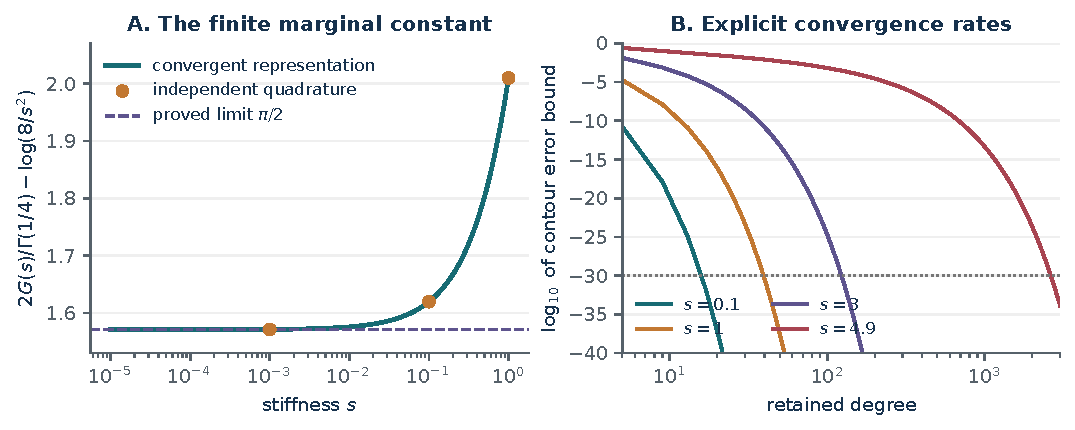
\includegraphics[width=\linewidth]{../figures/continuum_accuracy.pdf}
\caption{Left: the normalized finite part tends to $\pi/2$; the
markers are independent polylogarithm quadrature. Right: the proved
contour bound shows rapid convergence inside the disk and slower
convergence near its boundary. Curves are evaluations of the analytical
formulas, not fitted error models.}
\label{fig:continuum}
\end{figure}

The test suite contains 42 passing checks covering independent
representations, signed tails, exact coefficient zeros, inverse
residuals, enclosure widths, and failure at insufficient precision.
The symbolic recursion is checked exactly through degree six.
A root certificate produced using Corollary~\ref{cor:densitytemperature}
for $n_*=0.1$ and $\delta=0.01$ gives
\[
 T_{\con}=0.3595007501283353098918576878323848735202951682
 \quad\text{within }2\times10^{-46}.
\]
The full interval and its density calculation are saved in the certified
data. This uncertainty includes arithmetic rounding and the analytical
tail; it is not an estimate based only on a solver residual.

\subsection{Uniform lattice checks}

The lattice validator integrates the already subtracted $J-1$ expression
in energy-radial and Dirichlet coordinates. This avoids subtracting
two large densities near the marginal limit. It records an explicit
bound on omitted large-energy tails, and assesses quadrature sensitivity
by changing the quadrature order. The latter is a convergence diagnostic,
not an interval proof of quadrature error.

At $s=0$, understood as the regularized difference, the results are:

\begin{table}[ht]
\centering\small
\begin{tabular}{r r r}
\toprule
$T$ & $(N_{\latt}-N_{\con})/T^{3/2}$
& $((N_{\latt}-N_{\con})/T^{3/2}-\Bconst)/\sqrt T$\\
\midrule
$0.10$ & $0.00615630028566$ & $0.00307654039$\\
$0.05$ & $0.00585920488505$ & $0.00302223412$\\
$0.02$ & $0.00560536047131$ & $0.00298362066$\\
$0.01$ & $0.00548013858365$ & $0.00296725793$\\
\midrule
Predicted limit & $\Bconst=0.00518341279103$
& $\Dconst=0.00293576106393$\\
\bottomrule
\end{tabular}
\caption{The first two uniform lattice coefficients. All displayed
digits are numerical diagnostics; consult the data file for the
coarse--fine differences and omitted-tail bounds.}
\label{tab:lattice}
\end{table}

Crossovers at $s=0.01,0.1,1,10$ are also included. The largest scaled
coarse--fine discrepancy in those recorded tests is approximately
$3.24\times10^{-7}$. The explicit omitted-tail bound in the test setup
is below $2.4\times10^{-16}$; these are separate error quantities.

\begin{figure}[ht]
\centering
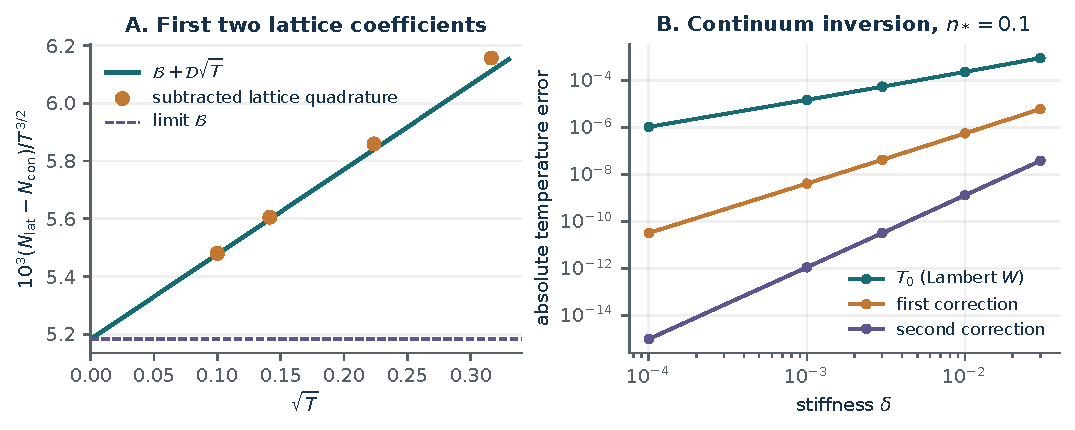
\includegraphics[width=\linewidth]{../figures/lattice_and_inverse.pdf}
\caption{Left: the regularized lattice difference approaches its
predicted two-term expansion. Right: the continuum inverse improves
when the first and second stiffness corrections are included. These
panels concern different asymptotic scales; the lattice theorem
explains their ordering.}
\label{fig:lattice}
\end{figure}

\subsection{How to reproduce the package}

The package root contains the article, code, tests, generated figures,
and machine-readable data. The reference implementation requires
\texttt{mpmath}; symbolic coefficient generation uses \texttt{sympy};
the lattice quadrature uses \texttt{numpy} and \texttt{scipy}; plots use
\texttt{matplotlib}; the certified evaluator uses
\texttt{python-flint 0.9.0}. Exact environment versions are recorded
in the supplied environment report.

From the package root, the principal commands are:
\begin{verbatim}
python3 -m pytest -q
python3 code/bose_certified.py 0.1 --atol 1e-30
python3 code/bose_certified.py --validation data/certified_validation.json
python3 code/validate_independent.py
python3 code/lattice_validate.py
python3 code/make_figures.py
cd article
latexmk -xelatex -interaction=nonstopmode marginal_bose_crossover.tex
\end{verbatim}
The independent quadrature is intentionally slower than the evaluator.
The README provides the exact commands and optional arguments for each
script. Numerical checks never replace the proof of a contour
displacement, the sharp radius, or the uniform lattice remainder.

\section{Proof audit, limitations, and interpretation}
\label{sec:audit}

\paragraph{What the result strengthens.}
Equation (25) of \cite{LJ2020} gives the correct leading logarithm.
We do not identify that statement as erroneous. The improvement is the
evaluation of the next coefficient and replacement of the leading
approximation by an exact, effectively convergent representation. The
explicit error estimate and the lattice theorem then support further
quantitative conclusions.

\paragraph{The dangerous interchange of limits.}
Substituting $\Psi(0)$ in every summand makes the harmonic series diverge.
Conversely, applying the large-argument Bessel asymptotic to every term
when $s$ is small misses the transition region. The Mellin transform
handles that region without a freely chosen cutoff. In the lattice
proof, positive-degree moments eliminate the marginal divergence from
the remainder; this is why its constant is uniform in stiffness.

\paragraph{A convergent series versus a formal residue list.}
The far-left estimate \eqref{eq:blockbound} is essential. A formal
residue calculation could produce a convergent-looking series while
leaving an unexamined contour term. Here the contour term is bounded
explicitly and tends to zero on the stated interval. The separate
coefficient estimate proves the exact complex radius.

\paragraph{Numerical certification.}
An analytical remainder bound combined with ordinary floating-point
evaluation is not automatically a certified interval. The package
therefore distinguishes its \texttt{mpmath} output from its Arb balls.
Quadrature refinement is reported as numerical evidence. Only the
enclosure implementation claims to include rounding in its interval.
A concrete numerical issue arose in the reference implementation:
very small Hurwitz-zeta values can lose relative accuracy before
multiplication by large gamma factors. The code evaluates
$\zeta(p,a)$ with an additional $\lceil p\log_{10}a\rceil+20$
digits and includes a regression check. The Arb implementation uses
the proved adaptive prefix allocation and rejects requested accuracies
unless the final ball radius meets the tolerance. In particular,
overlap alone is never accepted as an independent certificate.

\paragraph{Model dependence.}
The continuum constant pertains to the explicitly normalized crossover
integral. The coefficients $\Bconst$ and $\Dconst$ pertain to
\eqref{eq:latticedispersion}. A different lattice with the same leading
exponents can have different higher-order coefficients. The physical
mean-field interpretation does not prove the same formulas for a gas
with arbitrary short-range interactions, nor for the quantum
Heisenberg ferromagnet. Those questions require additional estimates
controlling interactions.

\paragraph{Priority and research status.}
The literature review located the precise leading law being
strengthened and related Mellin--Bessel technology. It did not locate
the complete specialized statement proved here. That is a bounded
literature finding, not a proof of publication priority. The package is
a research draft with analytical proofs and independent computational
checks, suitable for further mathematical review. No Lean or other
kernel-checked formalization is included.

\section{Further research questions}
\label{sec:future}

The following questions follow directly from the established formulas.
They are arranged so that the first few can be attacked without
introducing an interacting many-body theory.

\begin{enumerate}[label=\textbf{\arabic*.},leftmargin=*]
\item \textbf{Locate and classify the nearest complex singularities.}
The coefficient theorem proves the sharp radius $R_*$. Determine the
singularity type at each point on that circle and construct analytic
continuation across the remaining arcs. The late coefficient factor
$\cos(\pi k/4)$ gives specific directional information, but a complete
singularity theorem requires more than the radius calculation.

\item \textbf{Develop a joint expansion of every lattice coefficient.}
Use \eqref{eq:generalmellin} to obtain exact expansions of $C_r(s)$,
including the $s^r\log s$ terms. Establish coefficient bounds uniform
in $r$ sufficient to control a joint limit in $T$ and $s$, rather than
only each fixed order of the lattice expansion.

\item \textbf{Higher-order soft directions.}
Replace $x^4+s x^2$ by $x^{2m}+\sum_{j<m}s_jx^{2j}$ and place the
remaining directions at a marginal weighted dimension. Determine
finite constants, resonance logarithms, and convergence regions for
several stiffness parameters. The relevant critical points of the
polynomial suggest a geometric description of the convergence boundary.

\item \textbf{Nonseparable quartic forms.}
Study, for example, $x^2+y^4+z^4+\eta y^2z^2+\delta z^2$ with a
positive quartic form. Identify which parts of the marginal constant
have a closed form, and prove uniformity as the quartic form itself
approaches degeneracy. The separable gamma products used here will
need replacement by controlled angular integrals.

\item \textbf{A complete bit-complexity theorem.}
Charge the cost of gamma, zeta, logarithm, scaled Bessel evaluation,
and input/output precision. Investigate whether all necessary
half-integer zeta values can be generated together efficiently.
The special-function count in Theorem~\ref{thm:complexity} is a useful
starting point, but is not this stronger theorem.

\item \textbf{Certified lattice inversion and optimal evaluation near $R_*$.}
The continuum density-to-temperature certificate is already supplied
by Corollary~\ref{cor:densitytemperature}. Extend this approach to
$T_{\latt}$ using certified quadrature. Compare the simple two-regime scheme with
rational approximants or contour deformations. Any improved method
should preserve an explicit global error certificate.

\item \textbf{Finite-size crossover.}
Introduce finite periodic lengths in the soft directions and track
the joint limits of temperature, stiffness, and volume. Poisson
summation can connect the present heat-kernel approach to the Casimir
questions in \cite{LJ2020,PruszczykJakubczyk2023}; the zero mode must
be kept separate from the thermodynamic density.

\item \textbf{Universality under controlled lattice perturbations.}
Replace the exact sine-coordinate model by a class of analytic
nonnegative lattice symbols sharing the same leading weighted jet.
State and prove conditions under which the logarithmic constant is
unchanged and compute how the first lattice correction changes.
Uniform control of the complement of the minimum is necessary.

\item \textbf{Interactions beyond the mean-field model.}
Determine whether a rigorously bounded self-energy or effective
dispersion approximation preserves the marginal constant or only the
leading logarithm. A useful first target would be an explicit bound
comparing the interacting density to the ideal density on the scale
of $T^{3/2}$, with stiffness dependence stated rather than suppressed.

\item \textbf{Formal verification of the analytic core.}
Separate a potential formalization into the positive-integral
identities, Mellin inversion and contour displacement, gamma/zeta
identities, and the explicit majorants. Formalizing only the algebra
of the residues would leave the crucial equality and uniformity
questions unverified; the contour and domination arguments should
be explicit goals.
\end{enumerate}

\appendix
\section{Supplementary coefficient and inverse identities}

The coefficient formula \eqref{eq:stablecoeff} is preferable numerically
for $k\ge3$ because it uses zeta only at real arguments greater than
one. The eight-periodic cosine should be handled algebraically:
when $k\equiv2\pmod4$ the coefficient is exactly zero, subject to the
separate $k=2$ exception. Computing a tiny approximate cosine at a
mathematical zero would introduce spurious coefficients.

For example, the coefficient of $s^4$ in the normalized bracket is
\[
 b_4=\frac{\Gamma(9/4)}{24\Gamma(1/4)}\zeta(-1)
     =\frac{5}{384}\left(-\frac1{12}\right)=-\frac5{4608}.
\]
After multiplication by $8^2$, this becomes $d_4=-5/72$ in
\eqref{eq:firsttheta}. This cross-check distinguishes the two common
normalizations used in the report.

The recursion \eqref{eq:inverserecursion} also gives, with $D=w+1$,
\begin{equation}
 a_3=-\frac1D\left[
 a_1a_2-\frac{a_1^3}{6}
 +b_1\left(\frac{a_2}{2}-\frac{a_1^2}{8}\right)+b_3\right].
 \label{eq:a3}
\end{equation}
The $b_2z^2$ term has no $u$ dependence, because its exponent
$1-k/2$ is zero. This removes a possible source of an incorrect
second or third inverse coefficient. The accompanying symbolic
generator derives further coefficients from the exact implicit
equation and verifies their residuals.

\section{Source provenance and artifact notes}

The repository was inspected at commit
\begin{center}
\small\texttt{fd4aeeb2ee4fc729c18d98444fed42fd0529eeeb}.
\end{center}
The directly relevant source is Family 271, particularly the section
``The explicit lattice correction'' of
\emph{The first lattice correction to Bloch's law} \cite{OAIbloch}.
The article's independent mathematical target is the marginal
continuum formula in \cite{LJ2020}. Sources were checked on
8 October 2026. The source manifest records URLs and roles; no
third-party manuscript is repackaged as an original contribution.

The archive is self-contained for rebuilding this article once the
listed Python and LaTeX dependencies are installed. Data and figures
are generated artifacts; the analytical statements can be read and
checked without executing them. The PDF has been compiled and
visually reviewed. The complete validation outcome and the environment
are recorded separately so that the tests can be rerun after integration
into another repository.

\begin{thebibliography}{99}

\bibitem{LJ2020}
M. Łebek and P. Jakubczyk,
\emph{Dimensional crossovers and Casimir forces for the Bose gas in
anisotropic optical lattices}, Physical Review A \textbf{102} (2020),
013324. \href{https://doi.org/10.1103/PhysRevA.102.013324}{doi:10.1103/PhysRevA.102.013324}.
\href{https://arxiv.org/abs/2003.07458}{arXiv:2003.07458}, version 3,
especially Section IV.2 and equations (22)--(25).

\bibitem{FGD1995}
P. Flajolet, X. Gourdon, and P. Dumas,
\emph{Mellin transforms and asymptotics: harmonic sums},
Theoretical Computer Science \textbf{144} (1995), 3--58.
\href{https://doi.org/10.1016/0304-3975(95)00002-E}{doi:10.1016/0304-3975(95)00002-E}.
\href{https://specfun.inria.fr/dumas/Publications/FlGoDu95.pdf}{Author-hosted text}.

\bibitem{Paris2020}
R. B. Paris,
\emph{An expansion for the sum of a product of an exponential and a
Bessel function}, \href{https://arxiv.org/abs/1901.00142}{arXiv:1901.00142},
version 2 (2020).

\bibitem{LintonBarnett2004}
C. M. Linton and D. C. Barnett,
\emph{Efficient computation of Schlömilch-type series},
Proceedings of the Royal Society A \textbf{460} (2004), 1177--1191.
\href{https://doi.org/10.1098/rspa.2003.1202}{doi:10.1098/rspa.2003.1202}.

\bibitem{Corless1996}
R. M. Corless, G. H. Gonnet, D. E. G. Hare, D. J. Jeffrey, and D. E. Knuth,
\emph{On the Lambert $W$ function}, Advances in Computational
Mathematics \textbf{5} (1996), 329--359.
\href{https://doi.org/10.1007/BF02124750}{doi:10.1007/BF02124750}.
\href{https://cs.uwaterloo.ca/research/tr/1993/03/W.pdf}{Author-hosted text}.

\bibitem{DLMFgamma}
NIST Digital Library of Mathematical Functions,
\emph{Chapter 5: Gamma function}, especially Sections 5.4 and 5.5.
\url{https://dlmf.nist.gov/5.5}. Accessed 8 October 2026.

\bibitem{DLMFzeta}
NIST Digital Library of Mathematical Functions,
\emph{Section 25.4: Reflection formulas for the Riemann zeta function}.
\url{https://dlmf.nist.gov/25.4}. Accessed 8 October 2026.

\bibitem{PruszczykJakubczyk2023}
M. Pruszczyk and P. Jakubczyk,
\emph{Effective binding potential from Casimir interactions:
the case of the Bose gas},
\href{https://arxiv.org/abs/2211.06035}{arXiv:2211.06035} (2022), version 2.

\bibitem{OAIcatalog}
OpenAI, \emph{Mathematical manuscript collection and research catalog},
\url{https://github.com/openai/math}, Family 271. Repository commit
\texttt{fd4aeeb2ee4fc729c18d98444fed42fd0529eeeb}, inspected 8 October 2026.

\bibitem{OAIbloch}
OpenAI, \emph{The first lattice correction to Bloch's law},
manuscript dated 5 October 2026 in \texttt{openai/math}, Family 271.
\href{https://github.com/openai/math/blob/main/preprints/The-first-lattice-correction-to-Blochs-law-October-5-2026/first-lattice-correction-bloch-law.pdf}{Repository manuscript}.
Used for methodological inspiration only.

\bibitem{Arbdocs}
The python-flint developers,
\emph{python-flint 0.9.0 documentation: arb---real numbers}.
\url{https://python-flint.readthedocs.io/en/latest/arb.html}.
Accessed 8 October 2026.

\end{thebibliography}
\end{document}
